\section{Implementation details}
\label{sec:impl_details}

This section presents the datasets used for training and testing our method as well as insight about our implementation and a short presentation of the competitors compared to our proposal.

\subsection{Datasets}
\label{subsec:dataset}
	We have tested our proposal on the \textit{Oxford Robotcar} public dataset~\citep{Maddern2016} and on the \textit{CMU Visual localization} dataset~\citep{Bansal2014a} from the city of Pittsburg. These are common datasets used for image-based localization~\citep{Sattler2018} and loop closure algorithm involving neural networks training~\citep{Porav2018} under challenging conditions.
		
\paragraph{Training data.}
\label{para:training_data}
\begin{figure}
	\centering
	
	\begin{minipage}{0.5\linewidth}
		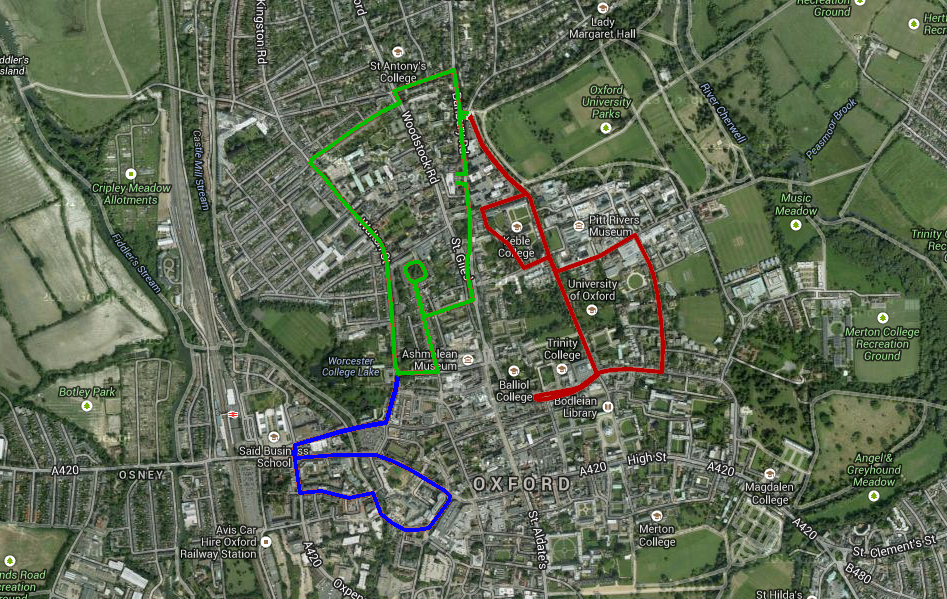
\includegraphics[width=\linewidth]{details/map}
	\end{minipage}\hfill	
	\begin{minipage}{0.5\linewidth}
		\caption[Data repartition]{\label{fig:data_repartition} \textbf{Train, validation and test zones:} the \textcolor{green}{green} path delimits our training area, the \textcolor{blue}{blue} trajectory the validation zone and the \textcolor{red}{red} path the test region. All the data are from the Oxford RobotCar dataset~\citep{Maddern2016}.}
	\end{minipage}

\end{figure}

We exploit the temporal redundancy present in Oxford Robotcar dataset to build the images triplets needed to train our CNN. We build 400 triplets using three runs acquired at dates: \texttt{15-05-19, 15-08-28} and \texttt{15-11-10}, and we select an area of the city different from the one used for training our networks for validation, see figure~\ref{fig:data_repartition}.

\begin{figure}

		\centering
		
		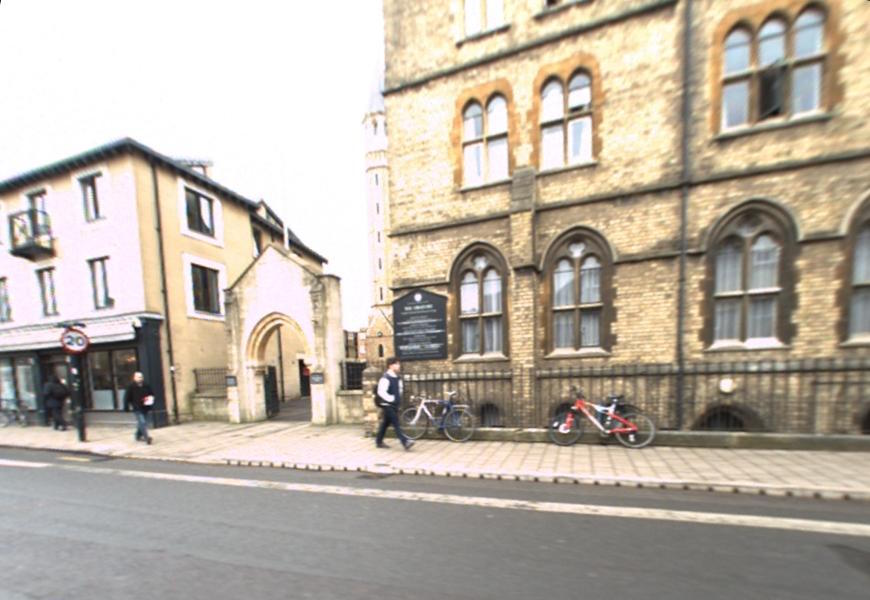
\includegraphics[width=0.33\linewidth]{details/image0.jpg}\hfill
		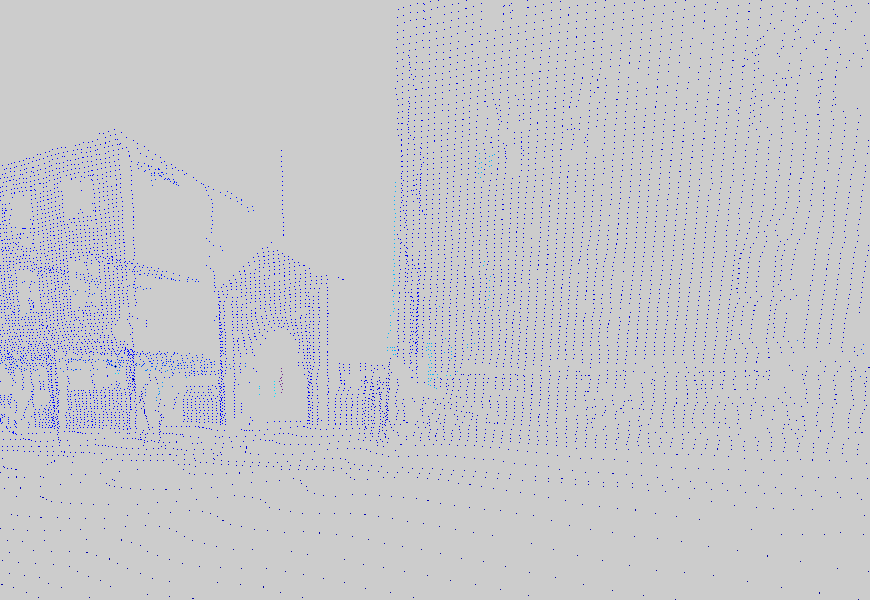
\includegraphics[width=0.33\linewidth]{details/sparsedepth0.png}\hfill
		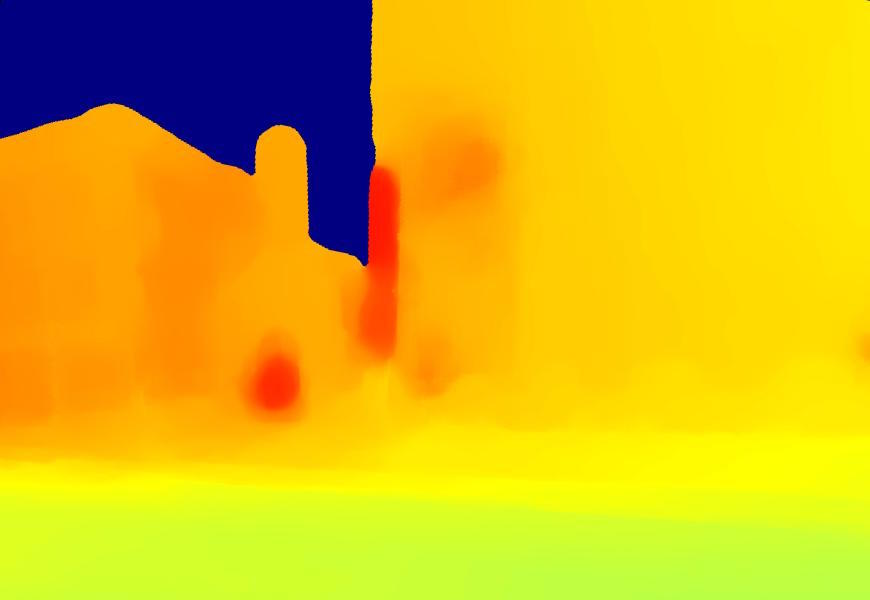
\includegraphics[width=0.33\linewidth]{details/densedepth0.jpg}\hfill
		
		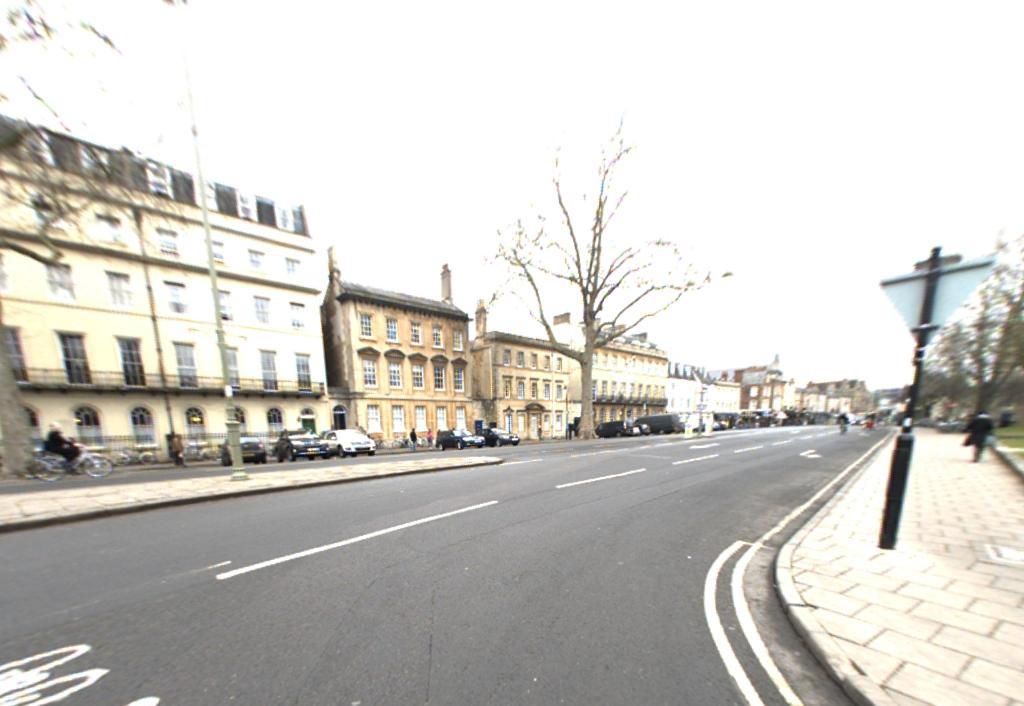
\includegraphics[width=0.33\linewidth]{details/image1.jpg}\hfill
		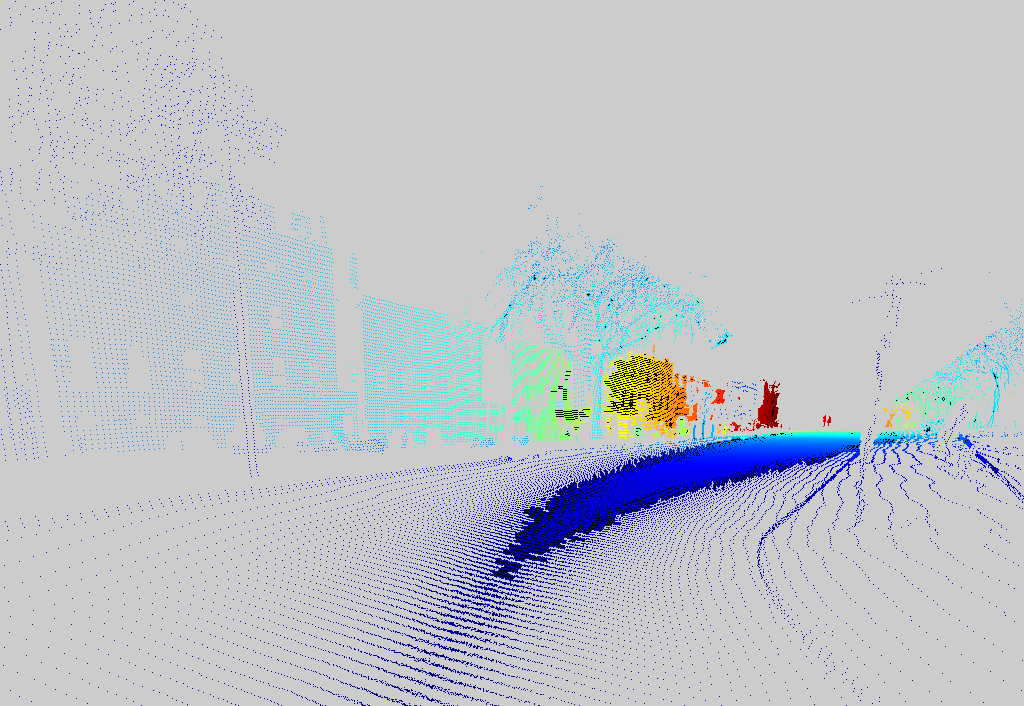
\includegraphics[width=0.33\linewidth]{details/sparsedepth1.png}\hfill
		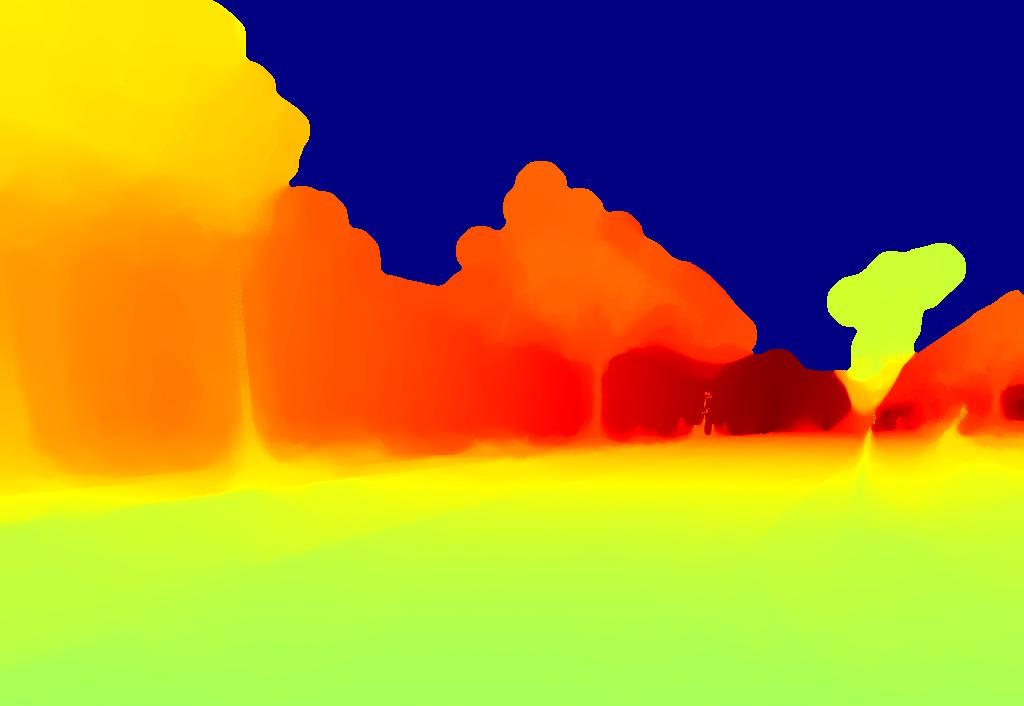
\includegraphics[width=0.33\linewidth]{details/densedepth1.jpg}\hfill
		\caption[Point cloud to depth map]{\label{fig:depth_map} \textbf{From point cloud to dense depth map:} from left to right: raw image, point cloud viewed from the camera frame, inpainted depth map by~\citep{Bevilacqua2017} (\textcolor{green}{green} is near, \textcolor{red}{red} is far).}

\end{figure}
	
Depth modality is extracted from the lidar point cloud. When re-projected in the image frame coordinate, it produces a sparse depth map. Since deep convolutional neural networks require dense data as input, we pre-process these sparse modality maps with the inpainting algorithm from~\citep{Bevilacqua2017} in order to make them dense. To avoid occlusion artifact (visible points that should not be visible because of occlusions) we use \ac{hpr} algorithm from~\citet{Katz2007} on the point cloud before further processing. We show in figure~\ref{fig:depth_map} example of depth maps generated through this pipeline. We drop depth values larger than 100 meters in order to produce depth maps with value in $[0, 1]$, consistent with the sigmoid decoder output (see annexe).

\paragraph{Testing data}
\begin{figure}
	\centering
	
	\begin{minipage}{0.435\linewidth}
		\includegraphics[width=\linewidth]{details/oxf_exs/ex1}
		
		\includegraphics[width=\linewidth]{details/oxf_exs/ex2}
		
		\includegraphics[width=\linewidth]{details/oxf_exs/ex4}
		
		\includegraphics[width=\linewidth]{details/oxf_exs/ex6}
		
		\includegraphics[width=\linewidth]{details/oxf_exs/ex3}
		
		\includegraphics[width=\linewidth]{details/oxf_exs/ex5}
		
		\scriptsize
		\begin{tabularx}
		{\linewidth}{X X X X}
			Reference images & 	Long-term & Snow queries & Night queries
		\end{tabularx}
	\end{minipage}\hfill	
	\begin{minipage}{0.555\linewidth}
		\includegraphics[width=\linewidth]{details/cmu_exs/ex1}
		
		\includegraphics[width=\linewidth]{details/cmu_exs/ex6}
		
		\includegraphics[width=\linewidth]{details/cmu_exs/ex4}	
		
		\includegraphics[width=\linewidth]{details/cmu_exs/ex2}	
		
		\includegraphics[width=\linewidth]{details/cmu_exs/ex3}	
		
		\includegraphics[width=\linewidth]{details/cmu_exs/ex5}	
		
		\scriptsize
		\begin{tabularx}{\linewidth}{X X X X}
			Reference images & Snow queries & Autumn queries & Long-term queries 
		\end{tabularx}
	\end{minipage}

	\caption[Examples of test images]{\label{fig:dataset} \textbf{Examples of test images :} we evaluate our proposal on 6 challenging localization sequences. Query image samples and the closest reference images in the database are presented from Oxford Robotcar~\cite{Maddern2016} (left) and CMU season dataset~\cite{Bansal2014a} (right).}
	
\end{figure}

We propose six testing scenarios, 3 on each datasets. For the Oxford Robotcar dataset, the reference dataset is composed of 1688 images taken every 5 meters along a path of 2 km, when the weather was overcast. The three query sets are:
\begin{itemize}
	\item {Oxford -- Long-term (LT):} queries have been acquired 7 months after the reference images under similar weather conditions,
	\item {Oxford -- Snow:} queries have been acquired during a snowy day,
	\item {Oxford -- Night:} queries have been acquired at night, resulting in radical visual changes compared to the reference images.
\end{itemize}

For the CMU Visual localization dataset, the reference dataset is composed of 1944 images with a sunny weather and the three query sets are:
\begin{itemize}
	\item {CMU -- Long-term (LT):} queries have been acquired 10 months after the reference images under similar weather conditions,
	\item {CMU -- Snow:} queries have been acquired during a snowy day,
	\item {CMU -- Autumn:} queries have been acquired during Autumn, featuring warm-coloured foliage and low sunlight compare to the reference data.
\end{itemize}

\noindent Query examples are presented in figure~\ref{fig:dataset}.
	
\paragraph{Evaluation metric}
For a given query, the reference images are ranked according to the cosine similarity score computed over their descriptors. To evaluate the localization performances, we consider two evaluation metrics:
\begin{itemize}
	\item \textbf{Recall @N:} we plot the percentage of well localized queries regarding the number $N$ of returned candidates. A query is considered well localized if one of the top $N$ retrieved images lies within $25m$ radius from the ground truth query position.
	\item \textbf{Top-1 recall @D:} we compute the distance between the top ranked returned database image position and the query ground truth position, and report the percentage of queries located under a threshold $D$ (from 15 to 50 meters), like in~\cite{Zamir2014}. This metric qualifies the accuracy of the localization system.
\end{itemize}


\subsection{Implementation}
\label{subsec:implementation}

Our proposal is implemented using Pytorch as deep learning framework, ADAM stochastic gradient descent algorithm for the CNN training with learning rate set to 1e-4, weight decay to 1e-3 and $\lambda$ in the triplet loss of equation~\ref{eq:triplet_loss} equal to 0.1. We use batch size between 10 and 25 triplets depending of the size of the system to train, convergence occurs rapidly and takes around 30 to 50 epochs. We perform hard negative mining as explained in section~\ref{subsec:hard_minning} with: $M_p \in [1, 4]$, $M_n^{sub} = 25$ and $M_n^{hard} = 10$. Positive examples are chosen within a radius of 7 meters around the anchor image  (according to GPS information) and we use the orientation given by position of the sensor on the Oxford mapping vehicle to ensure that cameras of positive examples are bearing in the same direction as the anchor camera (the vehicle is equipped with 4 cameras dispatched at the front, the back, the left side and the right side of the car). We set as negative examples data located further than 700 meters to the anchor. Images and depth maps are re-sized to $224\times224$ pixels before training and testing. 

\paragraph{Encoder architectures.}
We test the fully convolutional part of Alexnet~\citep{Krizhevsky2012} and Resnet18~\citep{he2016deep} (Resnet in short) architectures for features extraction. Weights are initialized with the pre-trained weights on ImageNet. We always use Alexnet encoder to extract features from raw depth map, reconstructed depth map, or hallucinated depth map. Indeed the quality of our depth map is usually very low, and we have found that using deeper network does not significantly improve localization results. We transform the 1-channel depth map into 3-channels jet colorization depth map in order to benefit from the convolutional filters learned on ImageNet. We do not use the 3-channels HHA depth map representation introduced in~\cite{Gupta2014} as it have been shown to perform equivalently to jet colorization~\cite{Eitel2015}.

\paragraph{Descriptor architectures.}
\begin{figure}
	\centering
	
	\begin{minipage}{0.4\linewidth}
		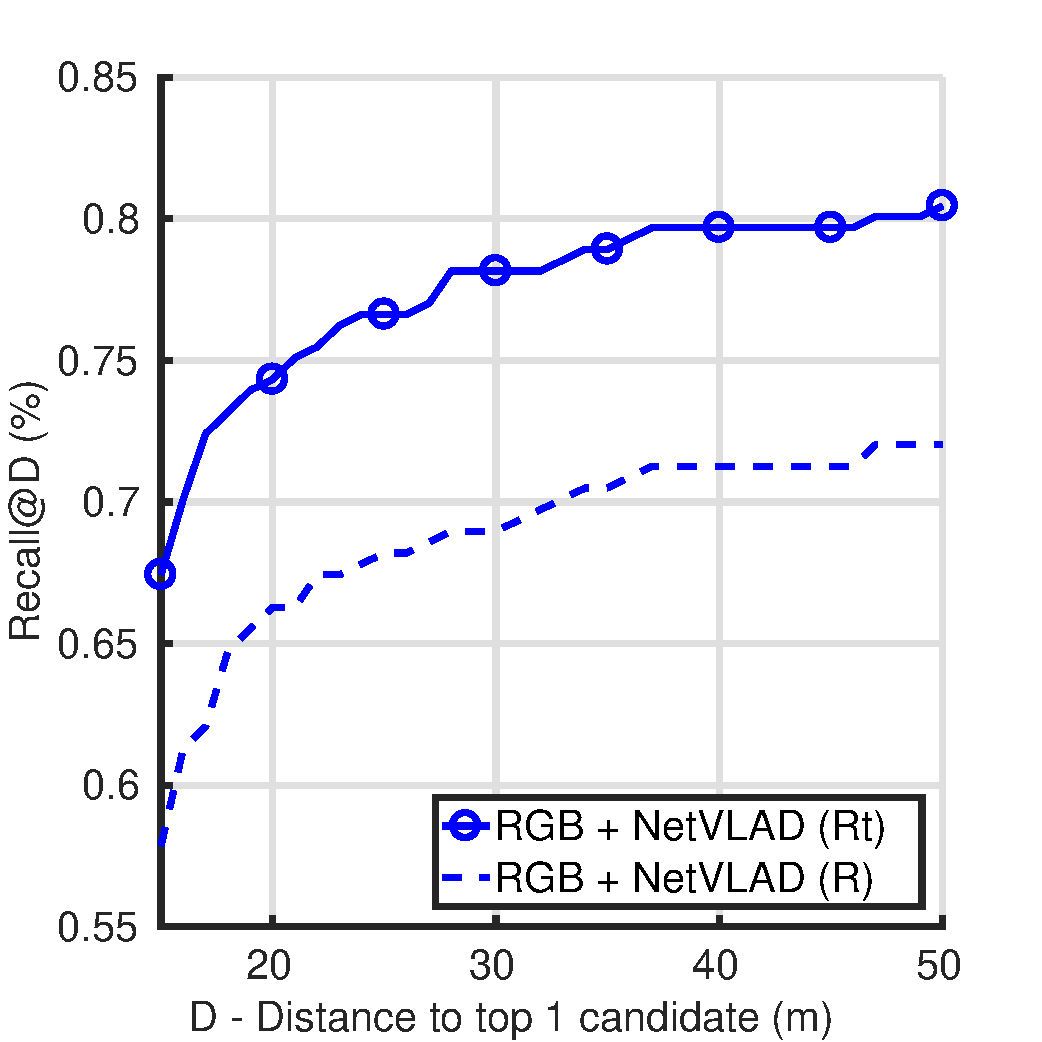
\includegraphics[width=\linewidth]{details/rgb_r_trunc_distance}	
	\end{minipage}
	\begin{minipage}{0.4\linewidth}
		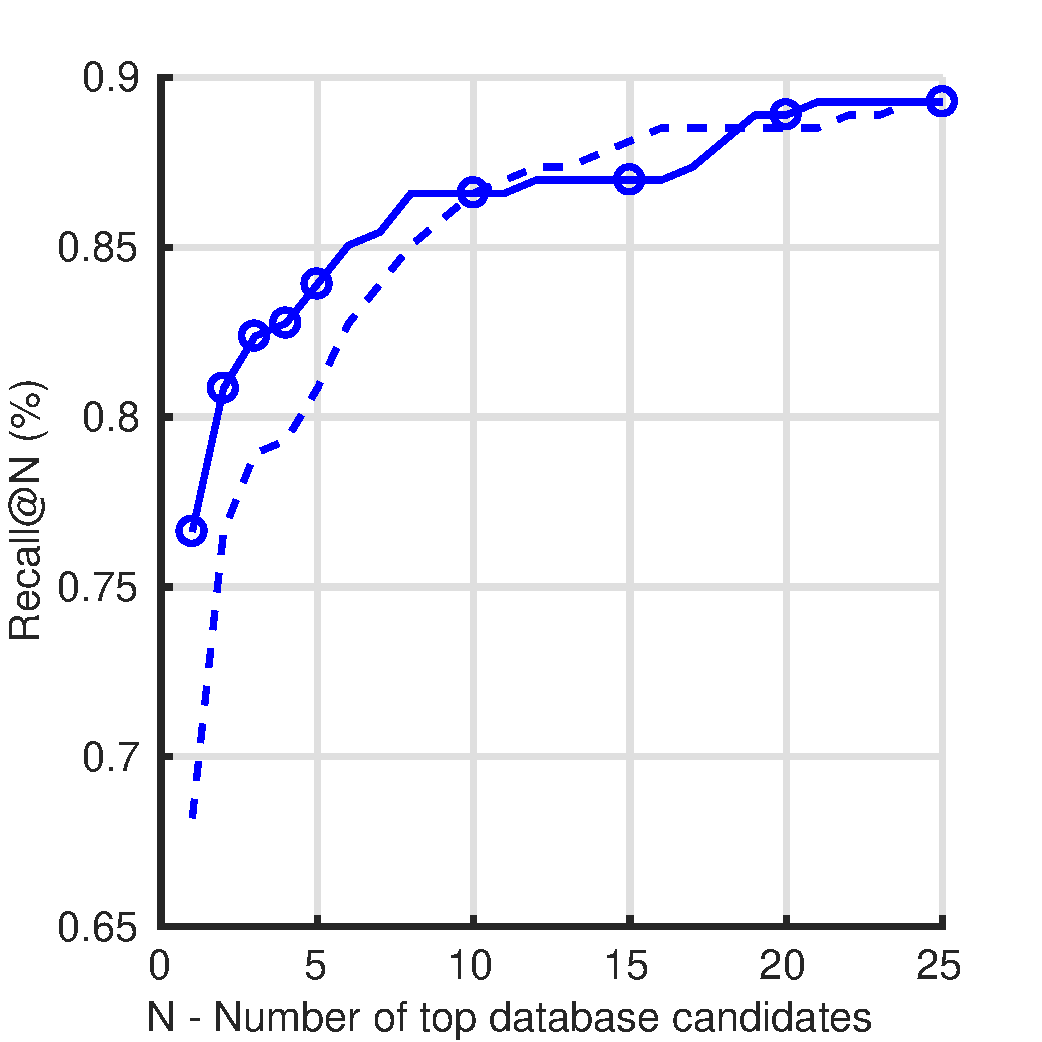
\includegraphics[width=\linewidth]{details/rgb_r_trunc_recall}	
	\end{minipage}
	
	\caption{\label{fig:trunc_resnet} \textbf{Full backbone Resnet18 versus truncated version in combination with NetVLAD :} we show the importance of the spatial resolution of the deep feature maps of the encoder used with NetVLAD layer. The truncated version of Resnet18 (Rt), more than two times lighter than the complete one (R), achieves much better localization results. Results are from only-RGB image descriptor~\citep{Arandjelovic2017}}
	
\end{figure}
We test the two state-of-the-art image descriptors MAC~\citep{Razavian2014a} and NetVLAD~\citep{Arandjelovic2017} (see section~\ref{sec:cbir_data_for_loc}). We experimented that NetVLAD descriptor combined with Resnet architecture does not perform well. NetVLAD can be view as a pooling method that acts on local deep features densely extracted from the input image. We argue that the spatial resolution of the features block obtained with Resnet encoder is too low compared to the other architecture (for instance $13\times13$ for Alexnet compared to $7\times7$ for Resnet for an $224\times224$ input image). We propose to use a truncated version of Resnet encoder, created by drooping the end of the network after the 13$^{th}$ convolutional layer. Thus we obtain a feature block with greater spatial resolution: $256\times14\times14$ compared to $512\times7\times7$. Results on our validation set for both architectures are presented in figure~\ref{fig:trunc_resnet}. As the truncated version of Resnet encoder clearly dominates the full one, we use the truncated version for the following experiments.

By combining Alexnet or Resnet encoder with MAC or NetVLAD descriptor pooling, we obtain 4 global image descriptor variants.

\paragraph{Decoder architecture.}
The decoder used in our proposal is based on Unet architecture and inspired by network generator from~\cite{Isola2017}. Dimension up-sampling is performed through inverse-convolutions layers. Decoder weights are initialized randomly.

\subsection{Competitors}
\label{subsec:competitors}
We compare the three following global image descriptors:
\begin{enumerate}
    \item \textit{RGB only (\textbf{RGB}):} simple networks composed of encoder + descriptor trained with images only, without side depth maps information. Networks are trained as explain in previous section, with triplet ranking loss of equation~\ref{eq:triplet_loss}. For fair comparison with our methods, we train the RGB network on the aforementioned dataset, but only with the radiometric modality.
    \item \textit{Our proposal (\textbf{RGB(D)}):} introduced in the previous section (see figure~\ref{fig:our_method}) this architecture uses pairs of aligned image and depth map during training step and images only at test time.
	\item \textit{Hallucination network (\textbf{RGB(H)}):} our version of the hallucination network~\cite{Hoffman2016} (see figure~\ref{fig:hall_method}), trained on aligned triplets of images and depth maps.
\end{enumerate}

For fair comparison, as \textbf{RGB(D)} and \textbf{RGB(H)} image descriptors are obtain by concatenation two full-size descriptors (see section~\ref{subsec:fuse_desc}), we perform PCA to reduce the size of the final descriptor of all three methods to 2048.